\section {DM Products} \label{sec:softproducts}
The DM products are not data as many may think, rather the products are software and services to produce those
products.
In operations DM will not exist though an analogous organization called Data Production will spring into existence under similar leadership.

The high level list of DM products is given in \figref{fig:pt}, as may be seen in the  figure we consider software, services and infrastructure as our categories of products.


\begin{figure}
\begin{centering}
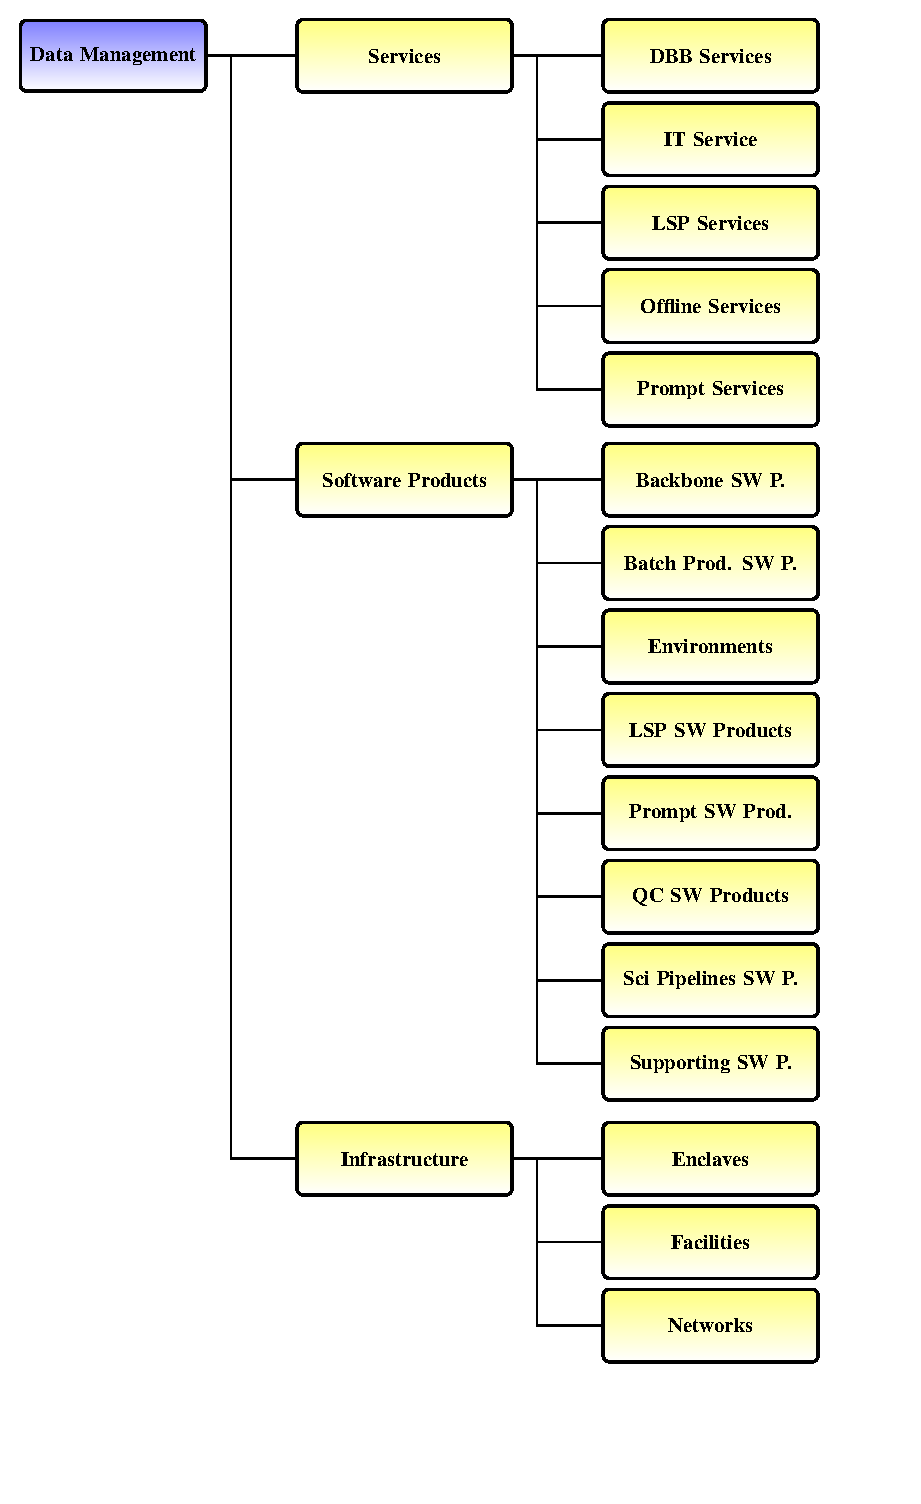
\includegraphics[width=0.7\textwidth]{images/ProductTree}
	\caption{Rubin DM product tree \label{fig:pt}}
\end{centering}
\end{figure}

It must be remarked that these products grew organically to some extent in a less than satisfactory manner.
As mentioned earlier some teams worked within their WBS area and produced planning and products without necessarily paying a lot of attention to other WBS elements. Hence we have some services which are really deployments of software produced by another team e.g Prompt Services and Prompt Software. But we do not always have a service for a piece of software though it may be web accessible and look like a service e.g. QC Products.
Some products are discussed in more below.


\subsection{Commissioning Software Products}
A detailed section describing what we delivered and used to process the commissioning data.
This section will probably not be written until  commissioning.

\subsection{Anticipated Data Release 1 Software Products}
A short section describing what we anticipate delivering  for DR1 in addition to what was delivered in commissioning.
This section will probably not be written until after commissioning.

\subsection{Science Platform}\label{sec:sciplat}
The science platform came into existence as a concept around the end of 2016, there had always been requirements to allow near the data processing and to  bring the code to the data but no concrete idea of how to do this. Of course Ipython notebooks were an obvious tool for a python based project but the advent of  Jupyter Hub  (2015) lead to a more client server notion much more online with bringing code to data. The first version of the science platform vision\cite{LSE-319} was created in 2017.

\begin{figure}
\begin{centering}
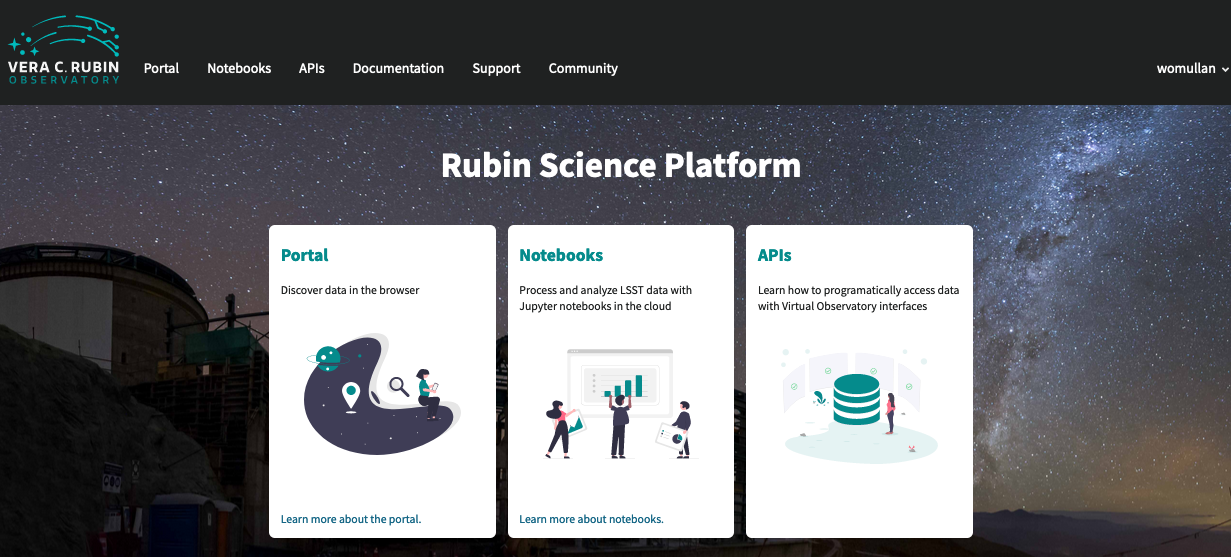
\includegraphics[width=0.4\textwidth]{images/datacloud}
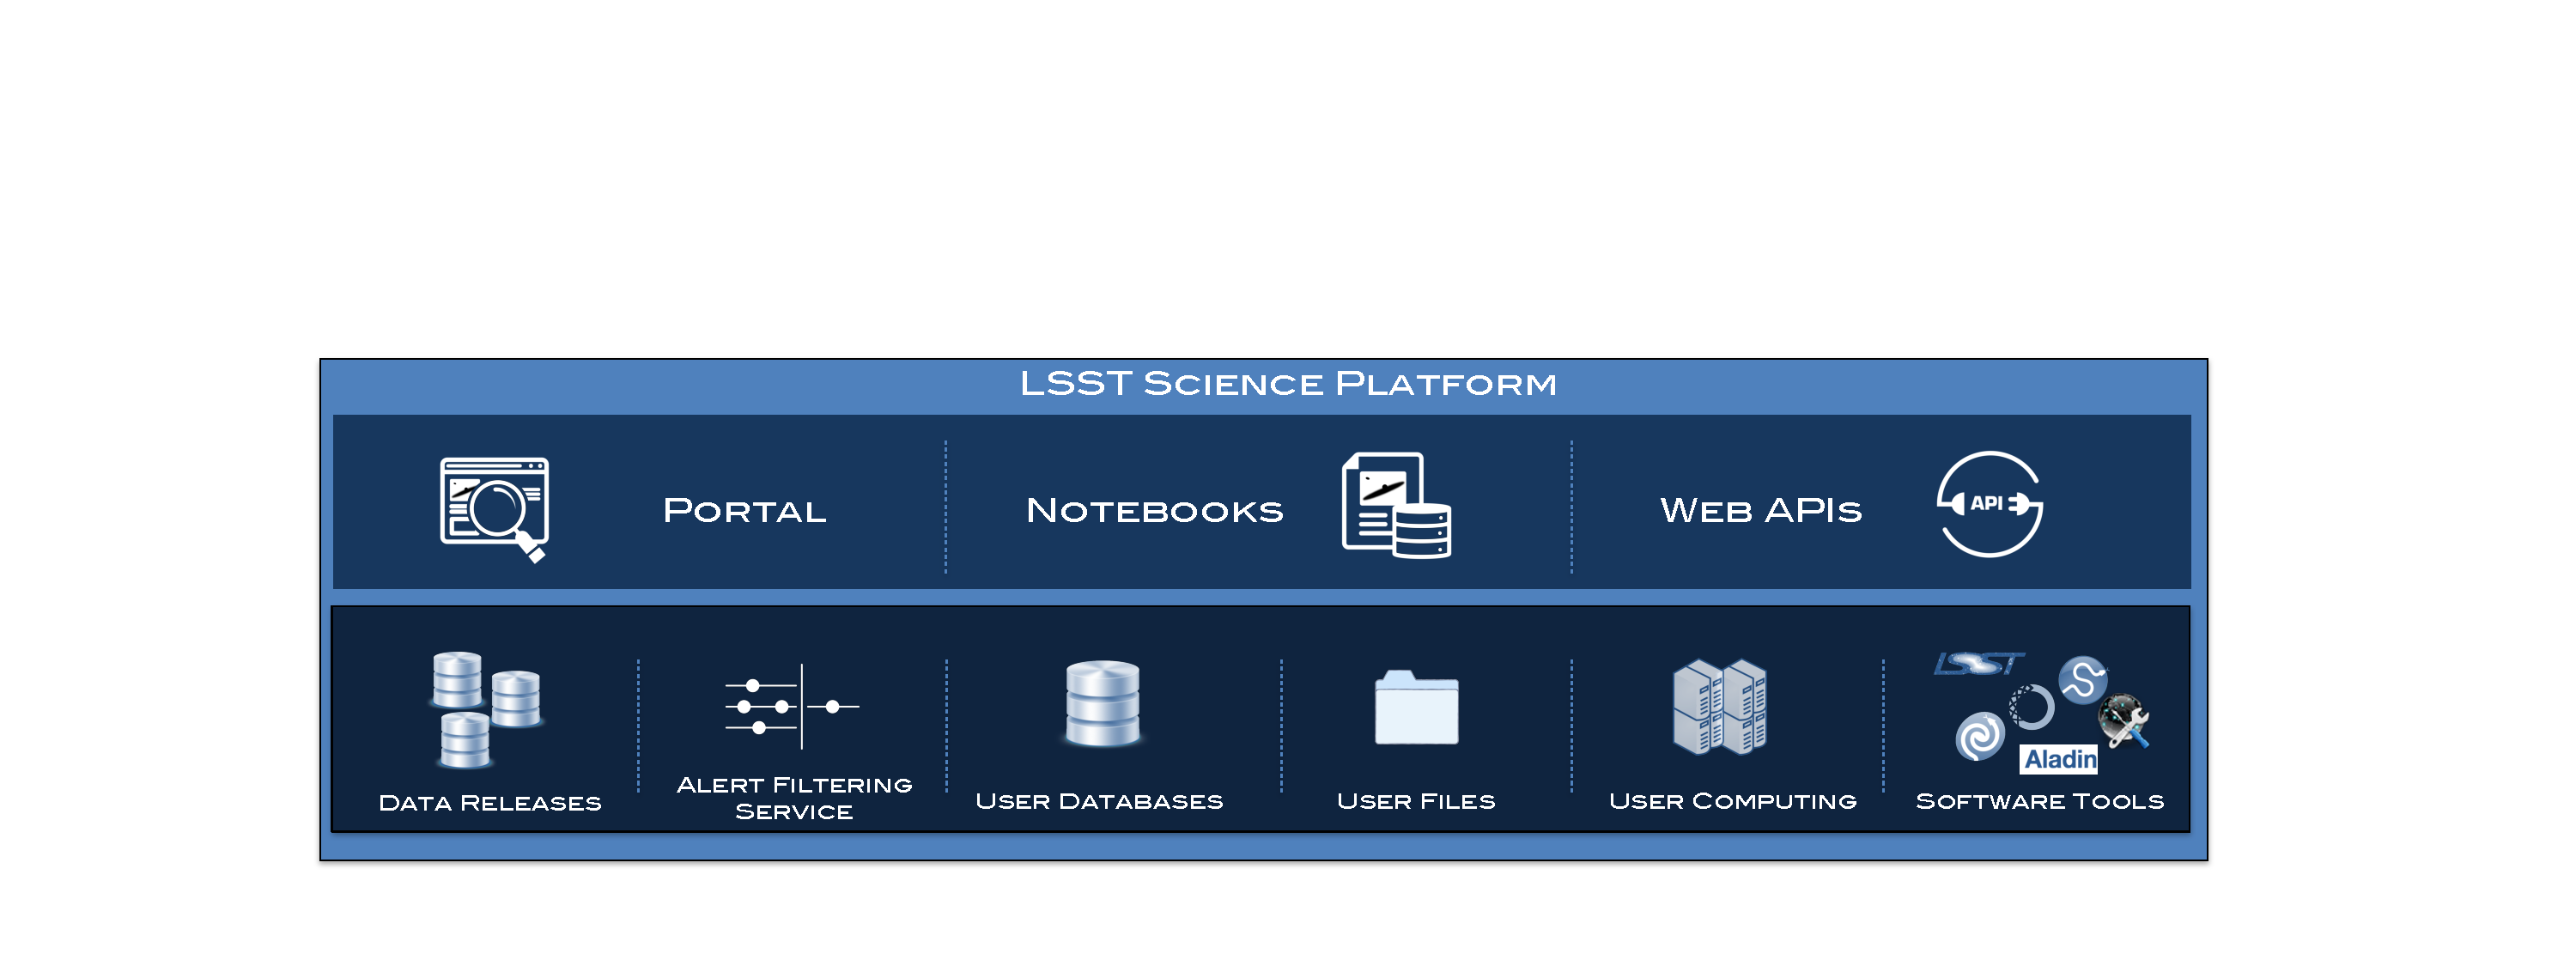
\includegraphics[width=0.4\textwidth]{images/fig-lsst-science-platform}
	\caption{Rubin Science platform as released in 2021(left) and components(right) \label{fig:sciplat}}
\end{centering}
\end{figure}

\subsection{Science Pipelines}\label{sec:pipes}
The science pipelines which produce the prompt and data release products are of course the most identifiable
software product from DM.
The detailed approach to Science Pipelines is covered in \cite{PSTN-019}.



\subsection{Services}

\subsection{Infrastructure}
